\subsection{Ensemble methods}

To improve the tree-based models, we used \textit{bagging} with 500 trees and afterwards \textit{random forest}, looking for the best value of \textit{m} predictors chosen among the full set of \textit{p} predictors. 

In figure \Fig~\ref{fig:m_best_for_500_plot} we can see the trend of the test and the out-of-bag error rates for increasing values of \textit{m}.

\begin{figure}[h]
	\centering
	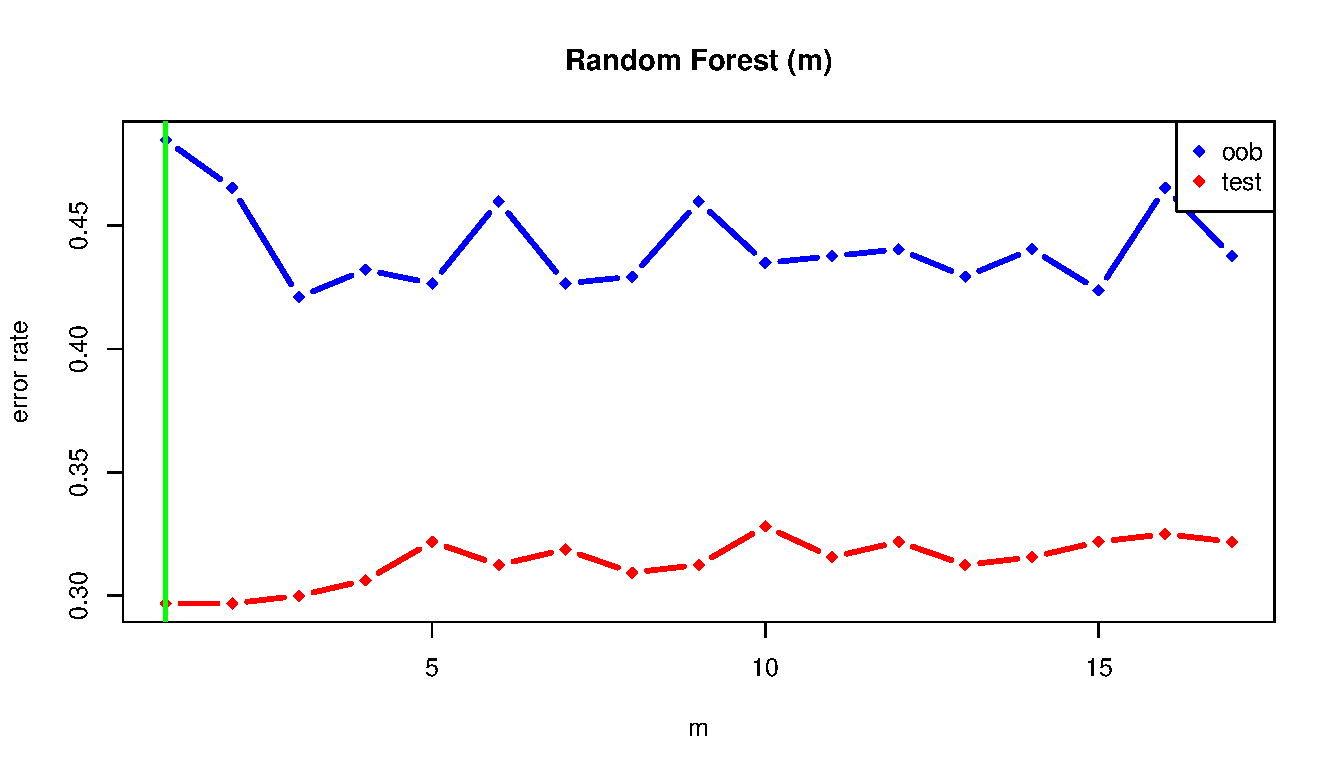
\includegraphics[width=0.5\linewidth]{ImageFiles/Classification/Trees/m_best_for_500_plot}
	\caption{Test and out-of-bag trends}
	\label{fig:m_best_for_500_plot}
\end{figure}

Computed the best \textit{m} for random forest (which gives the least test error rate), we made a comparison between the bagging model and the random forest one obtained with that particular value of \text{m}, keeping all the other parameters the same.
In figure \Fig~\ref{fig:vs_bagg_for_500_plot} we can see that the random forest perform slightly better than the bagging.

\begin{figure}[H]
	\centering
	\begin{subfigure}{.3\textwidth}
		\centering
		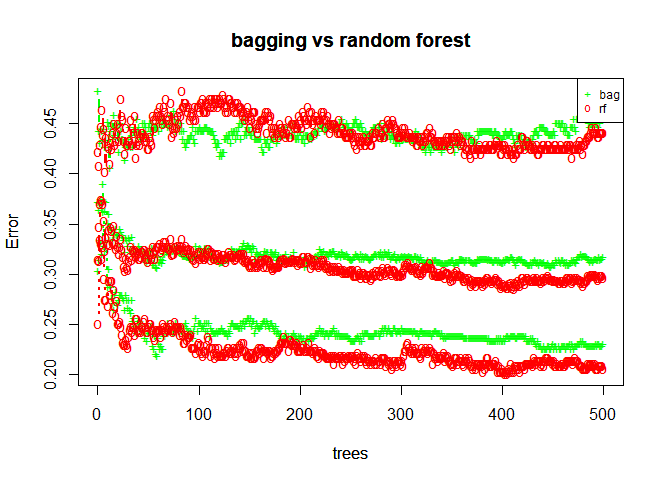
\includegraphics[width=\linewidth]{ImageFiles/Classification/Trees/vs_bagg_for_500_plot}
		\caption{Bagging and random forest comparison}
		\label{fig:vs_bagg_for_500_plot}
	\end{subfigure}%
	\hfill
	\begin{subfigure}{.3\textwidth}
		\centering
		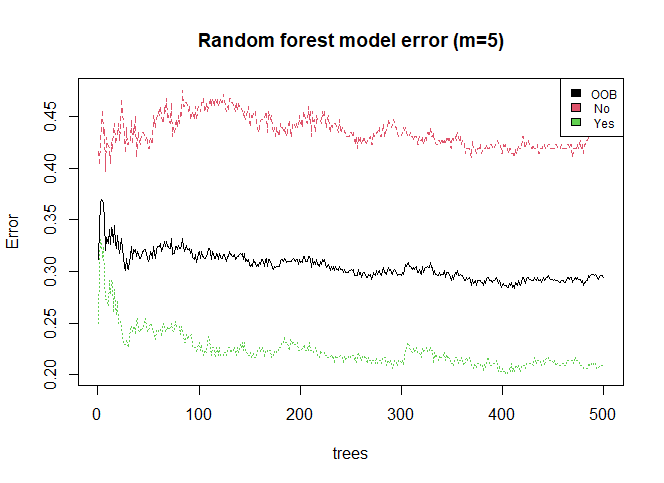
\includegraphics[width=\linewidth]{ImageFiles/Classification/Trees/best_for_500_plot}
		\caption{Random forest method plot (best m)}
		\label{fig:best_for_500_plot}
	\end{subfigure}%
	\hfill
	\begin{subfigure}{.3\textwidth}
		\centering
		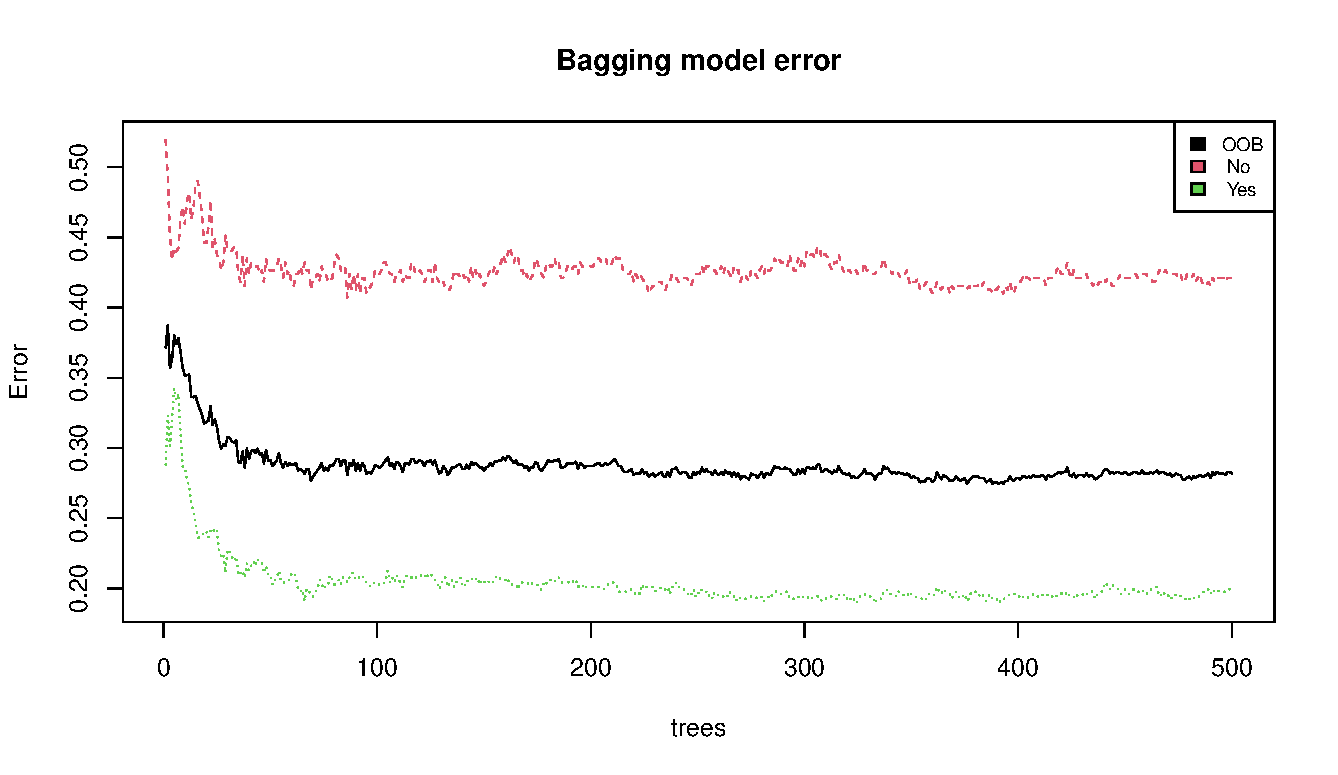
\includegraphics[width=\linewidth]{ImageFiles/Classification/Trees/bagg_500_plot}
		\caption{Bagging method plot}
		\label{fig:bagg_500_plot}
	\end{subfigure}
\end{figure}

We can obtain an overall summary of the importance of each predictor using RSS.
In figures \Fig~\ref{fig:best_for_500_var_imp_plot} and \Fig~\ref{fig:bagg_500_var_imp_plot} we can see the importance of each variable in each model.

\begin{figure}[h]
	\centering
	\begin{subfigure}{.5\textwidth}
		\centering
		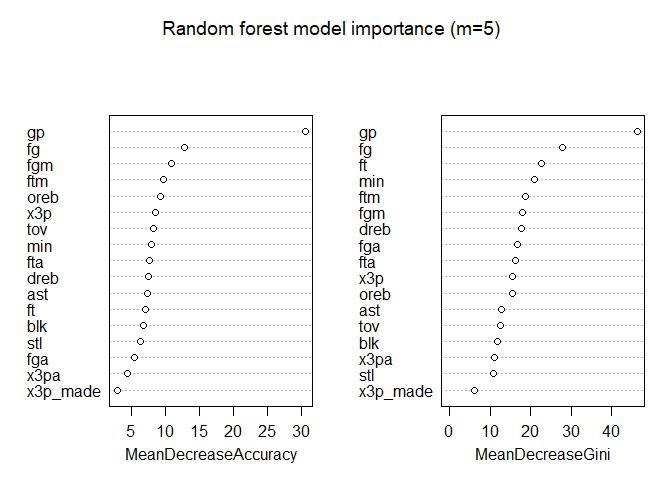
\includegraphics[width=0.5\linewidth]{ImageFiles/Classification/Trees/best_for_500_var_imp_plot}
		\caption{Random forest importance (best m)}
		\label{fig:best_for_500_var_imp_plot}
	\end{subfigure}%
	\hfill
	\begin{subfigure}{.5\textwidth}
		\centering
		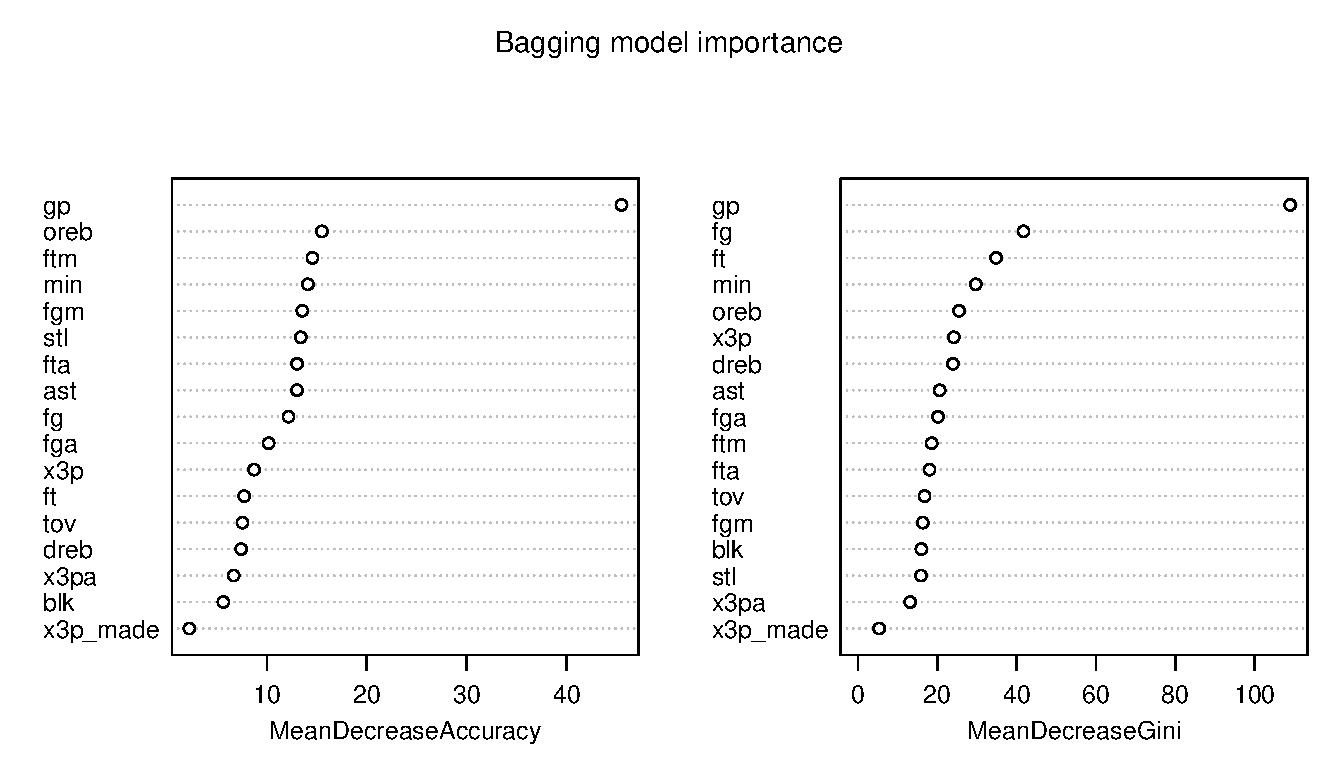
\includegraphics[width=0.5\linewidth]{ImageFiles/Classification/Trees/bagg_500_var_imp_plot}
		\caption{Bagging importance}
		\label{fig:bagg_500_var_imp_plot}
	\end{subfigure}
\end{figure}

\noindent
As in the classification trees, the \textit{gp} regressor is the most important one.

The goal of this section is to find the methodology that best fit our data at the cost of losing interpretability. For this purpose, we used \textit{boosting} in combination with cross-validation.

Many small trees were used with $\lambda = 0.001$: \Fig~\ref{fig:boost_4_rel_inf} shows the importance of each variable in the dataset given by the boosting technique.

\begin{figure}[H]
	\centering
	\begin{subfigure}{.5\textwidth}
		\centering
		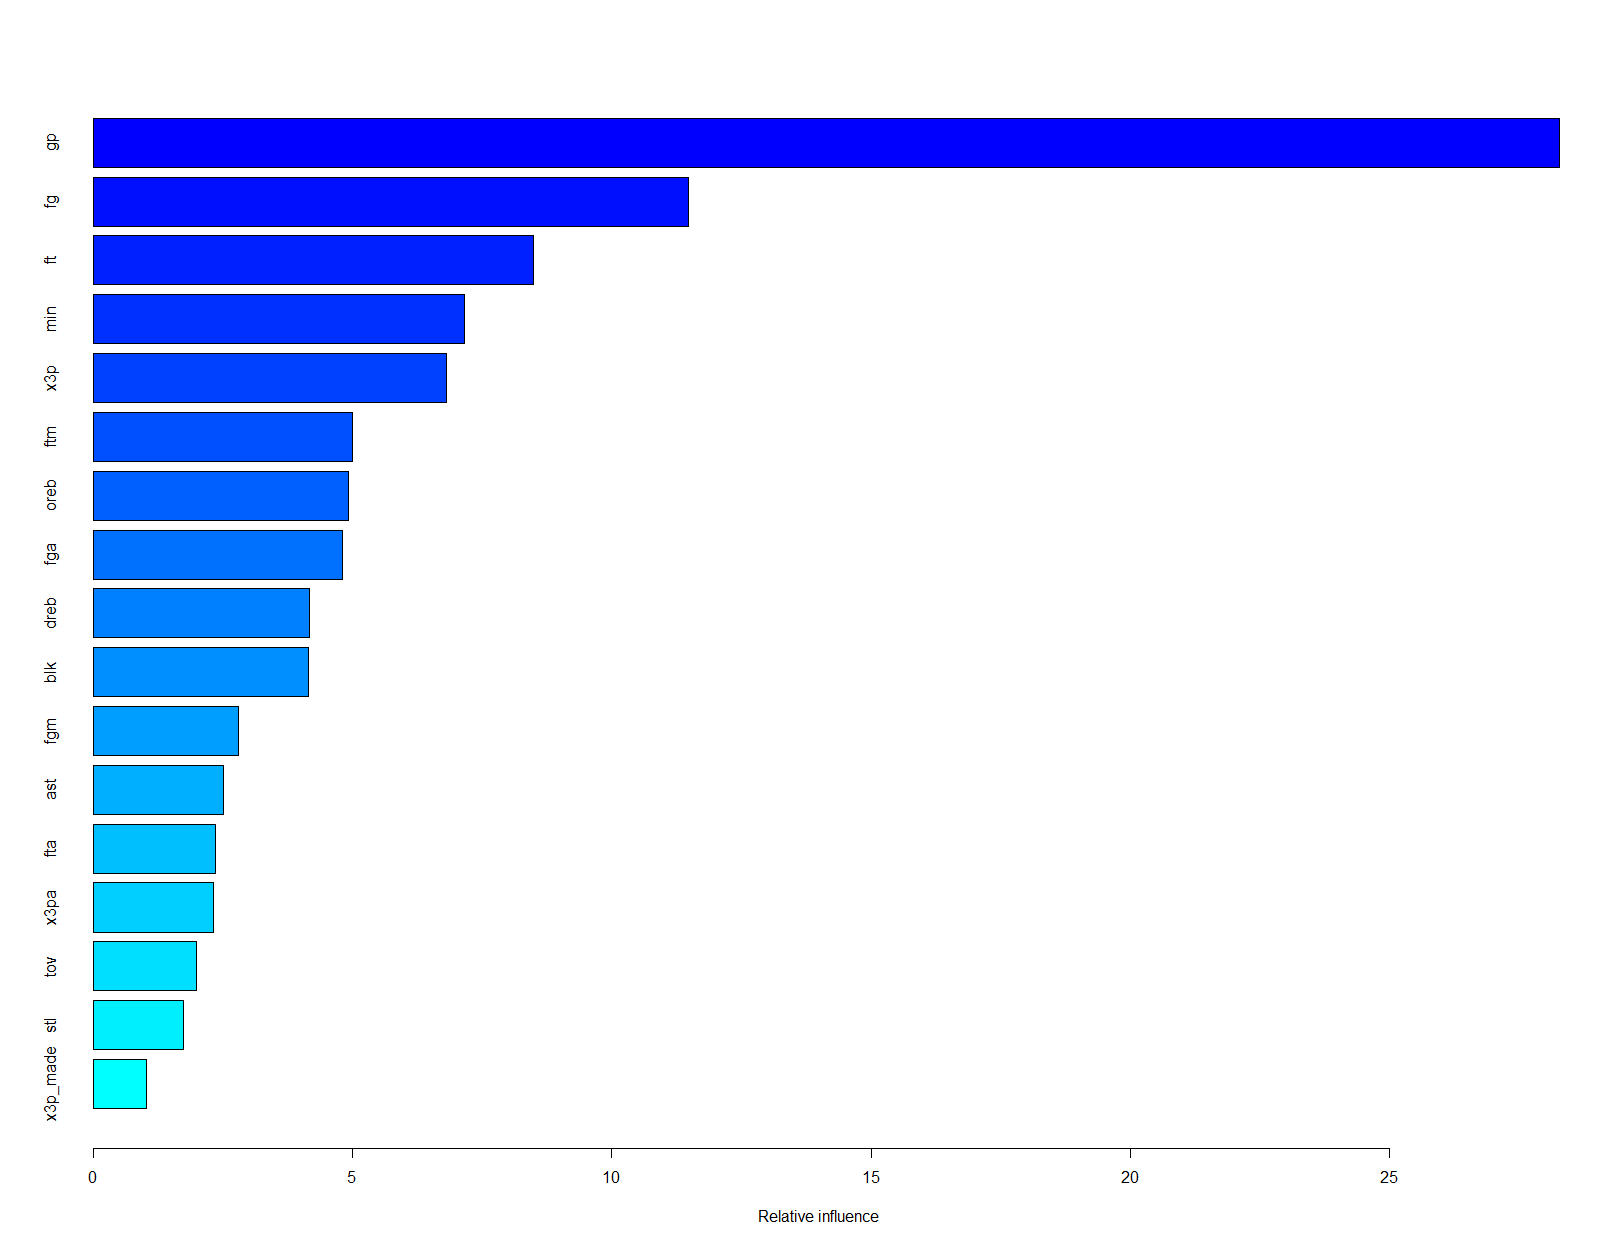
\includegraphics[width=0.6\linewidth]{ImageFiles/Classification/Trees/boost_4_rel_inf}
		\caption{Boosting relative influence}
		\label{fig:boost_4_rel_inf}
	\end{subfigure}%
	\hfill
	\begin{subfigure}{.5\textwidth}
		\centering
		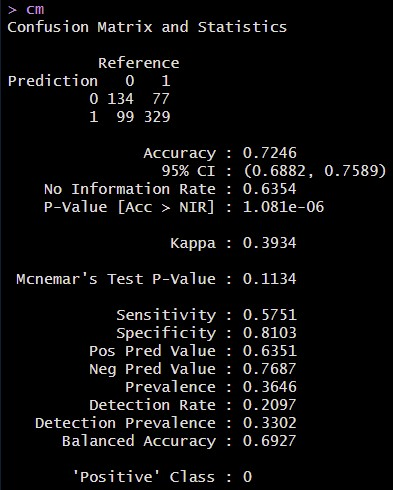
\includegraphics[width=0.4\linewidth]{ImageFiles/Classification/Trees/boost_4_conf_mat}
		\caption{Boosting confusion matrix}
		\label{fig:boost_4_conf_mat}
	\end{subfigure}
\end{figure}

As before, \textit{gp} is the most significant regressor.

